%&latex
\documentclass[12pt]{article}
\usepackage{amsmath}
\usepackage{graphicx,psfrag,epsf}
\usepackage{enumerate}
\usepackage{natbib}
\usepackage{url} % not crucial - just used below for the URL

% Additional packages
\usepackage{algorithm2e}
\usepackage{hyperref}

% Setup hyperlinks
\hypersetup{
  colorlinks=true,
  linkcolor=blue,
  citecolor=blue,      
  urlcolor=blue 
}

%\pdfminorversion=4
% NOTE: To produce blinded version, replace "0" with "1" below.
\newcommand{\blind}{0}

%
\newcommand{\pkg}[1]{\texorpdfstring%
{{\normalfont\fontseries{b}\selectfont #1}}%
{#1}}
\def\code#1{\texttt{#1}}
\def\pkg#1{\textbf{\texttt{#1}}}
\def\ref#1{\textbf{(#1)}}
\DeclareMathOperator{\flatness}{flatness}
\DeclareMathOperator{\imp}{imp}
\DeclareMathOperator{\inter}{int}

% DON'T change margins - should be 1 inch all around.
\addtolength{\oddsidemargin}{-.5in}%
\addtolength{\evensidemargin}{-.5in}%
\addtolength{\textwidth}{1in}%
\addtolength{\textheight}{1.3in}%
\addtolength{\topmargin}{-.8in}%


\begin{document}

%\bibliographystyle{natbib}

\def\spacingset#1{\renewcommand{\baselinestretch}%
{#1}\small\normalsize} \spacingset{1}


%%%%%%%%%%%%%%%%%%%%%%%%%%%%%%%%%%%%%%%%%%%%%%%%%%%%%%%%%%%%%%%%%%%%%%%%%%%%%%

\if0\blind
{
  \title{\bf A General Model-Based Variable Importance Metric for Supervised Learning}
  \author{Brandon M. Greenwell\thanks{
    The authors gratefully acknowledge \textit{please remember to list all relevant funding sources in the unblinded version}}\hspace{.2cm}\\
    Department of XXX, University of XXX\\
    and \\
    Andrew J. McCarthy \\
    Department of YYY, University of WWW \\
    and \\
    Bradley C. Boehmke \\
    Department of ZZZ, University of WWW }
  \maketitle
} \fi

\if1\blind
{
  \bigskip
  \bigskip
  \bigskip
  \begin{center}
    {\LARGE\bf Title}
\end{center}
  \medskip
} \fi

\bigskip
\begin{abstract}
In the era of "big data", it is becoming more of a challenge to not only build state-of-the-art predictive models, but also gain an understanding of what's really going on in the data. For example, it is often of interest to know which, if any, of the predictors in a fitted model are relatively influential on the predicted outcome. Fortunately, there are a few modern algorithms---like random forests and boosted decision trees---that have a natural way of ranking predictors in terms of some measure of importance or relative influence. Other algorithms---like neural networks and support vector machines---are not capable of doing so and model-free approaches are generally used to measure each predictors importance. In this paper, we discuss a model-based approach to measuring predictor importance in any supervised learning setting.
\end{abstract}

\noindent%
{\it Keywords:}  3 to 6 keywords, that do not appear in the title
\vfill

\newpage
\spacingset{1.45} % DON'T change the spacing!


%%%%%%%%%%%%%%%%%%%%%%%%%%%%%%%%%%%%%%%%%%%%%%%%%%%%%%%%%%%%%%%%%%%%%%%%%%%%%%%%
\section{Introduction}
\label{sec:introduction}
%%%%%%%%%%%%%%%%%%%%%%%%%%%%%%%%%%%%%%%%%%%%%%%%%%%%%%%%%%%%%%%%%%%%%%%%%%%%%%%%

Complex supervised learning algorithms, like neural networks and support vector machines, are more common than ever in predictive analytics, especially when dealing with large observational databases that don't adhere to the strict assumptions imposed by traditional statistical techniques (e.g., multiple linear regression which typically assumes linearity, homoscedasticity, and normality). However, it can be challenging to understand the results of such complex models and explain them to management. Graphical displays such as variable importance plots (when available) and partial dependence plots (PDPs) offer a simple solution. 

PDPs are low-dimensional graphical renderings of the prediction function $\widehat{f}\left(\boldsymbol{x}\right)$ so that the relationship between the outcome and predictors of interest can be more easily understood. These plots are especially useful in explaining the output from black box models. While PDPs can be constructed for any predictor in a fitted model, variable importance scores are more difficult to define. What does it mean for a feature to be important? It's influence on the predicted outcome? Some methods---like random forests and other tree-based methods---have a natural way of defining variable importance. Unfortunately, this is not the case for other popular supervised learning algorithms like support vector machines. In this paper, we consider a partial dependence-based variable importance metric that can be used with any supervised learning algorithm.


%%%%%%%%%%%%%%%%%%%%%%%%%%%%%%%%%%%%%%%%%%%%%%%%%%%%%%%%%%%%%%%%%%%%%%%%%%%%%%%%
\section{Background}
\label{sec:background}
%%%%%%%%%%%%%%%%%%%%%%%%%%%%%%%%%%%%%%%%%%%%%%%%%%%%%%%%%%%%%%%%%%%%%%%%%%%%%%%%

In the age of "big data", we are often confronted with the task of extracting knowledge from large databases. For this task we turn to various statistical learning algorithms which, when tuned correctly, can have state-of-the-art predictive performance. However, having a model that predicts well is only solving part of the problem. It is still necessary to extract information about the relationships uncovered by the learning algorithm. For instance, we often want to know which predictors, if any, are important by assigning some type of variable importance score to each feature. Once a set of influential features has been identified, the next step would be to summarize the functional relationship between each feature, or subset thereof, and the outcome of interest. However, since most statistical learning algorithms are "black box" models, extracting this information is not always straightforward. Luckily, some learning algorithms have a natural way of defining variable importance.


%%%%%%%%%%%%%%%%%%%%%%%%%%%%%%%%%%%%%%%%%%%%%%%%%%%%%%%%%%%%%%%%%%%%%%%%%%%%%%%%
\subsection{Model-based approaches to variable importance}
%%%%%%%%%%%%%%%%%%%%%%%%%%%%%%%%%%%%%%%%%%%%%%%%%%%%%%%%%%%%%%%%%%%%%%%%%%%%%%%%

In a binary decision tree, at each node $t$, a single predictor is used to partition the data into two homogeneous groups. The chosen predictor is the one that maximizes some measure of improvement $\widehat{i}_t$. The relative importance of predictor $x$ is just the sum of the squared improvements over all internal nodes of the tree for which $x$ was chosen as the partitioning variable; see \citet{classification-breiman-1984} for details. This idea also extends to ensembles of decision trees, like boosting and random forest. In ensembles, the improvement score for each predictor is averaged across all the trees in the ensemble. Fortunately, due to the stabilizing effect of averaging, the improvement-based variable importance metric is often more reliable in large ensembles \citep[pg. 368]{hastie-elements-2009}. Random forests offer an additional way to compute variable importance scores. The idea is to use the left over out-of-bag (OOB) data to construct validation-set errors for each tree. Then, each predictor is randomly shuffled in the OOB data and the error is computed again. The idea is that if variable $x$ is important, then the validation error will go up when $x$ is perturbed in the OOB data. The difference in the two errors is recorded for the OOB data then averaged across all trees in the forest.

In multiple linear regression, the absolute value of the $t$-statistic is commonly used as a measure of variable importance. The same idea also extends to generalized linear models and nonlinear least squares. Multivariate adaptive regression splines (MARS), which were introduced in \citet{friedman-1991-mars}, is an automatic and adaptive regression technique which can be seen as a generalization of multiple linear regression and generalized linear models. In the MARS algorithm, the contribution (or variable importance score) for each predictor is determined using a generalized cross-validation (GCV) statistic.

For neural networks, two popular methods for constructing variable importance scores are the Garson algorithm \citep{interpreting-garson-1991}, later modified by \citet{back-goh-1995}, and the Olden algorithm \citep{accurate-olden-2004}. Both algorithms use the network's connection weights to form the basis of the variable importance scores. The Garson algorithm determines variable importance by identifying all weighted connections between the nodes of interest. Olden's algorithm, on the other hand, uses the product of the raw input-hidden and hidden-output connection weights between each input and output neuron and sums the product across all hidden neurons. This has been shown to outperform the Garson method in various simulations.


%%%%%%%%%%%%%%%%%%%%%%%%%%%%%%%%%%%%%%%%%%%%%%%%%%%%%%%%%%%%%%%%%%%%%%%%%%%%%%%%
\subsection{Filter-based approaches to variable importance}
%%%%%%%%%%%%%%%%%%%%%%%%%%%%%%%%%%%%%%%%%%%%%%%%%%%%%%%%%%%%%%%%%%%%%%%%%%%%%%%%

Filter-based approaches, which are described in \citet[chap. 18]{applied-kuhn-2013}, do not make use of the fitted model to measure variable importance. They also do not take into account the other variables in the model.

For regression problems, a popular approach to measuring the variable importance of a numeric predictor $x$ is to first fit a flexible nonparametric model between $x$ and the target $Y$; for example, the locally-weighted polynomial regression (LOWESS) method of \citet{robust-cleveland-1979}. From this fit, a pseudo-$R^2$ measure can be obtained from the resulting residuals and used as a measure of variable importance. For categorical predictors, a different method based on standard statistical tests (e.g., $t$-tests and ANOVAs) are employed; see \citet[chap. 18]{applied-kuhn-2013} for details.

For classification problems, an area under the ROC curve (AUC) statistic can be used to quantify predictor importance. The AUC statistic is computed by using the predictor $x$ as input to the ROC curve. If $x$ can reasonably separate the classes of $Y$, then that is a clear indicator that $x$ is an important predictor (in terms of class separation) and this is captured in the corresponding AUC statistic. For problems with more than two classes, extensions of the ROC curve or a one-vs-all approach can be used.


%%%%%%%%%%%%%%%%%%%%%%%%%%%%%%%%%%%%%%%%%%%%%%%%%%%%%%%%%%%%%%%%%%%%%%%%%%%%%%%%
\subsection{Partial dependence plots}
%%%%%%%%%%%%%%%%%%%%%%%%%%%%%%%%%%%%%%%%%%%%%%%%%%%%%%%%%%%%%%%%%%%%%%%%%%%%%%%%

\citet{harrison-1978-hedonic} were among the first to analyze the well-known Boston housing data. One of their goals was to find a housing value equation using data on median home values from $n = 506$ census tracts in the suburbs of Boston from the 1970 census; see \citet[Table IV]{harrison-1978-hedonic} for a description of each variable. The data violate many classical assumptions like linearity, normality, and constant variance. Nonetheless, \citeauthor{harrison-1978-hedonic}---using a combination of transformations, significance testing, and grid searches---were able to find a reasonable fitting model ($R^2 = 0.81$). Part of the payoff for there time and efforts was an interpretable prediction equation which is reproduced in Equation~\eqref{eqn:boston}.
\begin{equation}
\label{eqn:boston}
\begin{aligned}
\widehat{\log\left(MV\right)} &= 9.76 + 0.0063 RM^2 + 8.98\times10^{-5} AGE - 0.19\log\left(DIS\right) + 0.096\log\left(RAD\right) \\
  & \quad - 4.20\times10^{-4} TAX - 0.031 PTRATIO + 0.36\left(B - 0.63\right)^2 - 0.37\log\left(LSTAT\right) \\
  & \quad - 0.012 CRIM + 8.03\times10^{-5} ZN + 2.41\times10^{-4} INDUS + 0.088 CHAS \\
  & \quad - 0.0064 NOX^2.
\end{aligned}
\end{equation}

Nowadays, many supervised learning algorithms can fit the data automatically in seconds---typically with higher accuracy. The downfall, however, is some loss of interpretation since these algorithms typically do not produce simple prediction formulas like Equation~\eqref{eqn:boston}. These models can still provide insight into the data, but it is not in the form of simple equations. For example, quantifying predictor importance has become an essential task in the analysis of "big data", and many supervised learning algorithms, like tree-based methods, can naturally assign variable importance scores to all of the predictors in the training data.

While determining predictor importance is a crucial task in any supervised learning problem, ranking variables is only part of the story and once a subset of "important" features is identified it is often necessary to assess the relationship between them (or subset thereof) and the response. This can be done in many ways, but in machine learning it is often accomplished by constructing \textit{partial dependence plots} (PDPs); see \citet{friedman-2001-greedy} for details. PDPs help visualize the relationship between a subset of the features (typically 1-3) and the response while accounting for the average effect of the other predictors in the model. They are particularly effective with black box models like random forests and support vector machines.

Let $\boldsymbol{x} = \left\{x_1, x_2, \dots, x_p\right\}$ represent the predictors in a model whose prediction function is $\widehat{f}\left(\boldsymbol{x}\right)$. If we partition $\boldsymbol{x}$ into an interest set, $\boldsymbol{z}_s$, and its compliment, $\boldsymbol{z}_c = \boldsymbol{x} \setminus \boldsymbol{z}_s$, then the "partial dependence" of the response on $\boldsymbol{z}_s$ is defined as
\begin{equation}
\label{eqn:avg_fun}
  f_s\left(\boldsymbol{z}_s\right) = E_{\boldsymbol{z}_c}\left[\widehat{f}\left(\boldsymbol{z}_s, \boldsymbol{z}_c\right)\right] = \int \widehat{f}\left(\boldsymbol{z}_s, \boldsymbol{z}_c\right)p_{c}\left(\boldsymbol{z}_c\right)d\boldsymbol{z}_c,
\end{equation}
where $p_{c}\left(\boldsymbol{z}_c\right)$ is the marginal probability density of $\boldsymbol{z}_c$: $p_{c}\left(\boldsymbol{z}_c\right) = \int p\left(\boldsymbol{x}\right)d\boldsymbol{z}_s$.
Equation~\eqref{eqn:avg_fun} can be estimated from a set of training data by
\begin{equation}
\label{eqn:pdf}
\bar{f}_s\left(\boldsymbol{z}_s\right) = \frac{1}{n}\sum_{i = 1}^n\widehat{f}\left(\boldsymbol{z}_s,\boldsymbol{z}_{i, c}\right),
\end{equation}
where $\boldsymbol{z}_{i, c}$ $\left(i = 1, 2, \dots, n\right)$ are the values of $\boldsymbol{z}_c$ that occur in the training sample; that is, we average out the effects of all the other predictors in the model.

Constructing a PDP \eqref{eqn:pdf} in practice is rather straightforward. To simplify, let $\boldsymbol{z}_s = x_1$ be the predictor variable of interest with unique values $\left\{x_{11}, x_{12}, \dots, x_{1k}\right\}$. The partial dependence of the response on $x_1$ can be constructed as follows:

\begin{algorithm}
\begin{enumerate}
  \item For $i \in \left\{1, 2, \dots, k\right\}$:
  \begin{enumerate}
    \item Copy the training data and replace the original values of $x_1$ with the constant $x_{1i}$.
    \item Compute the vector of predicted values from the modified copy of the training data.
    \item Compute the average prediction to obtain $\bar{f}_1\left(x_{1i}\right)$.
  \end{enumerate}
  \item Plot the pairs $\left\{x_{1i}, \bar{f}_1\left(x_{1i}\right)\right\}$ for $i = 1, 2, \dotsc, k$.
\end{enumerate}
\caption{A simple algorithm for constructing the partial dependence of the response on a single predictor $x_1$. \label{alg:pdp}}
\end{algorithm}
Algorithm~\eqref{alg:pdp} can be quite computationally intensive since it involves $k$ passes over the training records. Fortunately, the algorithm can be performed in parallel quite easily. It can also be easily extended to larger subsets of two or more features as well.


%%%%%%%%%%%%%%%%%%%%%%%%%%%%%%%%%%%%%%%%%%%%%%%%%%%%%%%%%%%%%%%%%%%%%%%%%%%%%%%%
\subsection{Boston housing data}
%%%%%%%%%%%%%%%%%%%%%%%%%%%%%%%%%%%%%%%%%%%%%%%%%%%%%%%%%%%%%%%%%%%%%%%%%%%%%%%%

For illustration, we will use a corrected version of the Boston housing data analyzed in \citet{harrison-1978-hedonic}; the data are available from Statlib at \url{http://lib.stat.cmu.edu/datasets/boston_corrected.txt}. Using the R package \pkg{randomForest} \citep{randomForest-pkg}, we fit a random forest with tuning parameter $m_{try} = 6$ (chosen using 5-fold cross-validation) and 1000 trees. The model fit is reasonable, with an \textit{out-of-bag} (pseudo) $R^2$ of 0.89. The variable importance scores are displayed in Figure~\ref{fig:boston-rf-vip}. Both plots indicate that the percentage of lower status of the population (\code{lstat}) and the average number of rooms per dwelling (\code{rm}) are highly associated with the median value of owner-occupied homes (\code{cmedv}). They also indicate that the proportion of residential land zoned for lots over 25,000 sq.ft (\code{zn}) has little association with \code{cmedv}.
\begin{figure}[!htb]
  \centering
  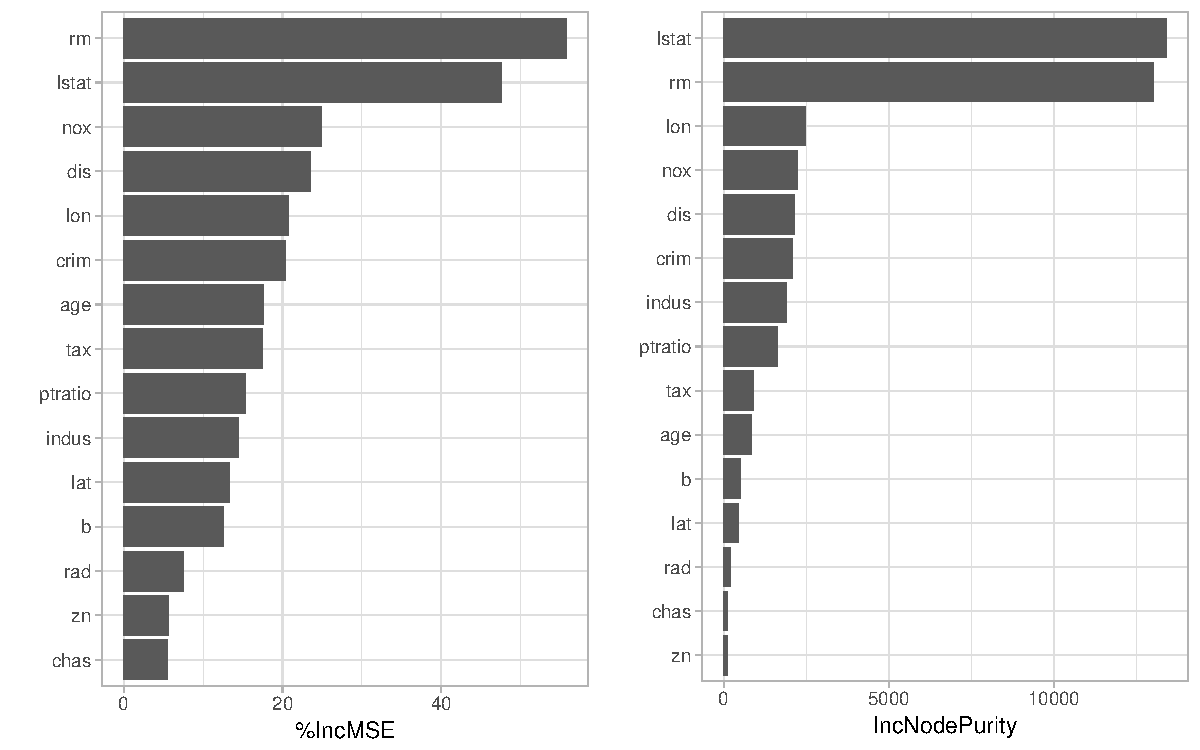
\includegraphics[width=1.0\textwidth]{boston-rf-vip}
  \caption{Variable importance scores from a random forest fit to the (corrected) Boston housing data. \textit{Left}: OOB-based variable importance scores. \textit{Right}: Impurity-based variable importance scores. \label{fig:boston-rf-vip}}
\end{figure}

The PDPs for these three variables are displayed in Figure~\ref{fig:boston-rf-pdps}. Notice how the PDP for \code{zn} is essentially flat, compared to the PDPs for \code{lstat} and \code{rm}. It is this notion of "flatness" which we will use as a basis to define our variable importance measure.
\begin{figure}[!htb]
  \centering
  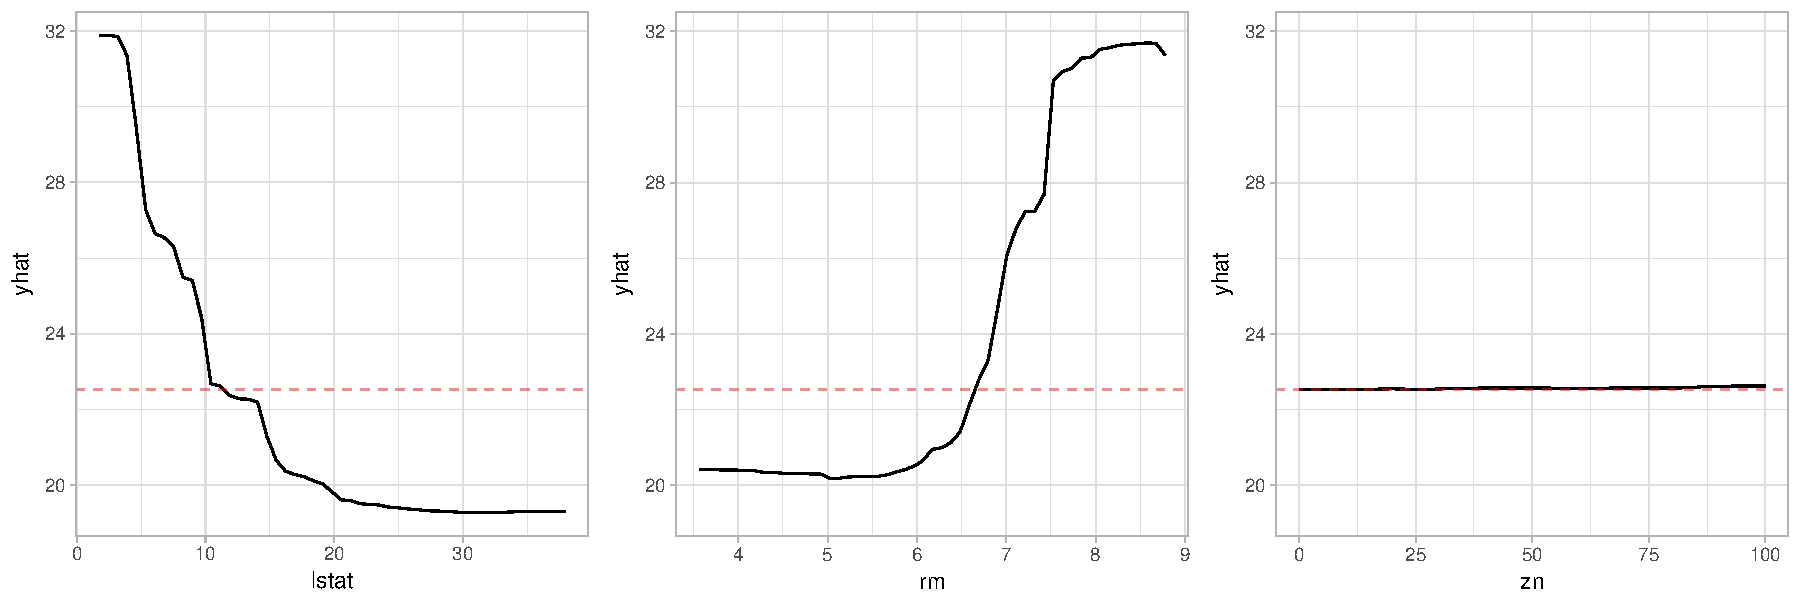
\includegraphics[width=1.0\textwidth]{boston-rf-pdps}
  \caption{Partial dependence of \code{cmedv} on \code{lstat} (left), \code{rm} (middle), and \code{zn} (right). The mean of the $n = 506$ median home values is indicated by a dashed red line. \label{fig:boston-rf-pdps}}
\end{figure}


%%%%%%%%%%%%%%%%%%%%%%%%%%%%%%%%%%%%%%%%%%%%%%%%%%%%%%%%%%%%%%%%%%%%%%%%%%%%%%%%
\section{A model-based variable importance measure}
\label{sec:new}
%%%%%%%%%%%%%%%%%%%%%%%%%%%%%%%%%%%%%%%%%%%%%%%%%%%%%%%%%%%%%%%%%%%%%%%%%%%%%%%%

The PDP for \code{zn} in Figure~\ref{fig:boston-rf-pdps} is relatively flat, indicating that \code{zn} does not have much influence on the predicted median home value. In other words, the partial dependence values $\bar{f}\left(x_{i}\right)$ $\left(i = 1, 2, \dots, k\right)$ display little variability. One might conclude that any variable for which the PDP is "flat" is likely to be less important than those predictors whose PDP varies across a wider range of the response.

Our notion of variable importance is based on any measure of the "flatness" of the partial dependence function. In general, we define
\begin{equation*}
  \imp\left(x\right) = \flatness\left(\bar{f}_s\left(\boldsymbol{z}_s\right)\right),
\end{equation*}
where $\flatness$ is any measure of "flatness" of the curve. A simple and effective measure to use is the sample standard deviation for continuous predictors and the range statistic (divided by 4) for factors with $K$ levels. Based on Algorithm~\eqref{alg:pdp}, our importance metric for predictor $x_1$ is simply
\begin{equation}
\label{eqn:vi-con}
  \imp\left(x_1\right) = \sqrt{\frac{1}{k - 1}\sum_{i = 1}^k\left[\bar{f}_1\left(x_{1i}\right) - \frac{1}{k}\sum_{i = 1}^k\bar{f}_1\left(x_{1i}\right)\right] ^ 2},
\end{equation}
if $x_1$ is continuous and
\begin{equation}
\label{eqn:vi-fac}
  \imp\left(x_1\right) = \left[\max_i\left(\bar{f}_1\left(x_{1i}\right)\right) - \min_i\left(\bar{f}_1\left(x_{1i}\right)\right)\right] / 4,
\end{equation}
if $x_1$ is categorical. Note that our variable importance metric relies on the fitted model; hence, it is crucial to properly tune and train the model to have good performance.

To illustrate, we apply Algorithm~\eqref{alg:pdp} to all of the predictors in the random forest for the Boston housing example and compute \eqref{eqn:vi-con}\footnote{We used Equation~\eqref{eqn:vi-fac} for \code{chas} since it is a categorical variable with two levels.}. The results are displayed in Figure~\ref{fig:boston-rf-vip-pd}. In this case, out partial dependence-based algorithm matches closely with the results from the random forest.

\begin{figure}[!htb]
  \centering
  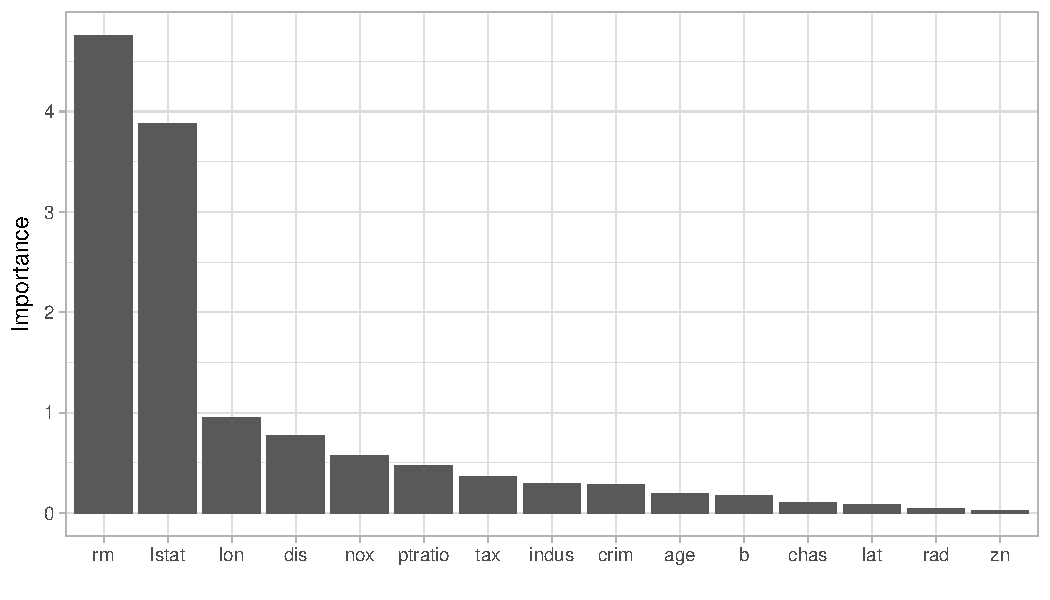
\includegraphics[width=1.0\textwidth]{boston-rf-vip-pd}
  \caption{Partial-dependence-based variable importance scores from a random forest fit to the (corrected) Boston housing data. \label{fig:boston-rf-vip-pd}}
\end{figure}


%%%%%%%%%%%%%%%%%%%%%%%%%%%%%%%%%%%%%%%%%%%%%%%%%%%%%%%%%%%%%%%%%%%%%%%%%%%%%%%%
\subsection{Linear models}
\label{sec:linear}
%%%%%%%%%%%%%%%%%%%%%%%%%%%%%%%%%%%%%%%%%%%%%%%%%%%%%%%%%%%%%%%%%%%%%%%%%%%%%%%%

As mentioned earlier, for linear models, a natural choice for measuring the importance of each term is to use the absolute value of the corresponding coefficient divided by its estimated standard error (i.e., the absolute value of the $t$-statistic). This turns out to be equivalent to the partial dependence-based metric \eqref{eqn:vi-con} when the predictors are independently and uniformly distributed over the same range.

For example, suppose we have a linear model of the form
\begin{equation*}
  Y = \beta_0 + \beta_1 X_1 + \beta_2 X_2 + \epsilon,
\end{equation*}
where $\beta_i$ ($i = 1, 2$) is a constant, $X_1$ and $X_2$ are both $\mathcal{U}\left(0, 1\right)$ random variables, and $\epsilon \sim \mathcal{N}\left(0, \sigma ^ 2\right)$. Since we know the distribution of $X_1$ and $X_2$, we can easily find $f_1\left(X_1\right)$ and $f_2\left(X_2\right)$. For instance, 
\begin{equation*}
  f_1\left(X_1\right) = \int_0^1 E\left[Y | X_1, X_2\right] p\left(X_2\right) dX_2,
\end{equation*}
where $p\left(X_2\right) = 1$. Simple calculus then leads to 
\begin{equation*}
  f_1\left(X_1\right) = \beta_0 + \beta_2 / 2 + \beta_1 X_1 \quad and \quad f_2\left(X_2\right) = \beta_0 + \beta_1 / 2 + \beta_2 X_2..
\end{equation*}
Since $E\left[Y | X_1, X_2\right] = f\left(X_1, X_2\right)$ is additive, the true partial dependence functions are just simple linear regressions in each predictor with their original coefficient and an adjusted intercept. Taking the variance of each gives
\begin{equation*}
Var\left[f_1\left(X_1\right)\right] = \beta_1 ^ 2 / 12 \quad and \quad Var\left[f_2\left(X_2\right)\right] = \beta_2 ^ 2 / 12.
\end{equation*}
Hence, the standard deviations are just the absolute values of the original coefficients (scaled by the same constant).

To illustrate, we simulated $n = 1000$ observations from the following linear model
\begin{equation*}
  Y = 1 + 3 X_1 - 5 X_2 + \epsilon,
\end{equation*}
where $X_1$ and $X_2$ are both $\mathcal{U}\left(0, 1\right)$ random variables, and $\epsilon \sim \mathcal{N}\left(0, 0.01 ^ 2\right)$. For this example, we have 
\begin{equation*}
  f_1\left(X_1\right) = -\frac{3}{2} + 3 X_1 \quad and \quad f_2\left(X_1\right) = \frac{5}{2} - 5 X_2.
\end{equation*}
These are plotted as red lines in Figure~\ref{fig:lm-pdps}. Additionally, the black lines in Figure~\ref{fig:lm-pdps} correspond to the estimated partial dependence functions using Algorithm~\eqref{alg:pdp}.

\begin{figure}[!htb]
  \centering
  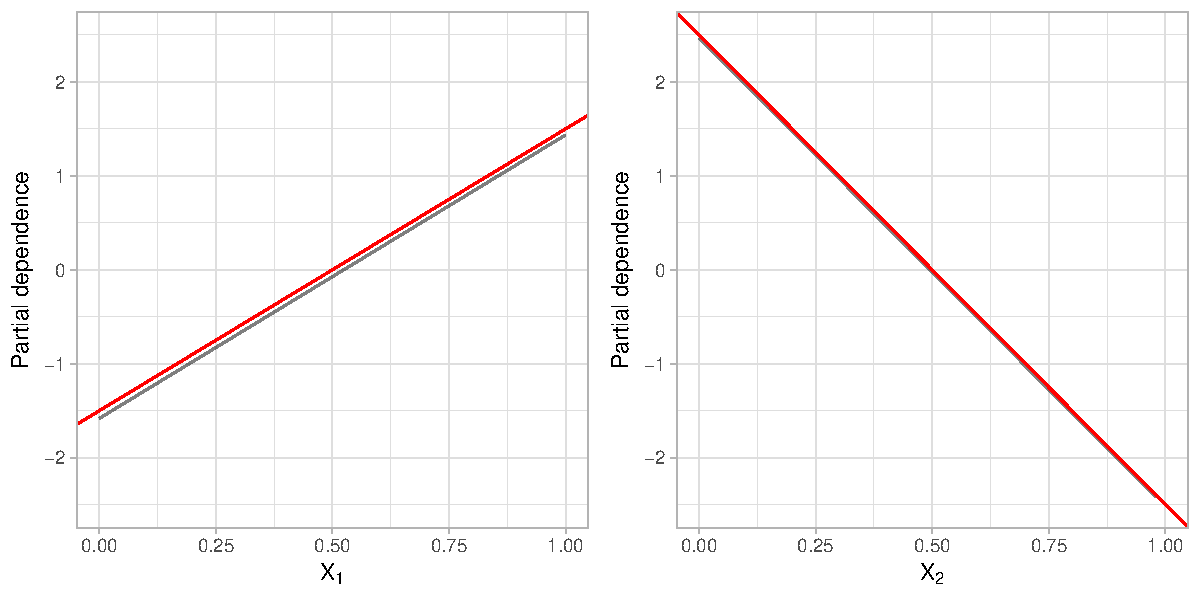
\includegraphics[width=1.0\textwidth]{lm-pdps}
  \caption{Estimated and true partial dependence plots. \label{fig:lm-pdps}}
\end{figure}

Clearly, $X_2$ is more influential than $X_1$. Taking the absolute value of the ratio of the slopes in $f_2\left(X_2\right)$ and $f_1\left(X_1\right)$ gives $5 / 3 \approx 1.67$. In other words, $X_2$ is roughly 1.67 times more influential on $Y$ than $X_1$. Using the partial-dependence-based variable importance metric, we obtain $\imp\left(X_1\right) = 1.4828203$ and $\imp\left(X_2\right) = 0.8961719$ which gives the ratio $\imp\left(X_2\right) / \imp\left(X_1\right) \approx 1.65$. In fact, we can compute the true variance for both partial dependence functions:
\begin{equation*}
Var\left[f_1\left(X_1\right)\right] = 3^2 / 12 \quad and \quad Var\left[f_2\left(X_2\right)\right] = 5^2 / 12.
\end{equation*}
Hence, the ratio of the true standard deviations is $5 / 3 \approx 1.67$.

Using the absolute value of the $t$-statistic becomes less useful in linear models when, for example, a predictor appears in multiple terms (e.g., interaction effects and polynomial terms). The partial dependence approach, on the other hand, does not suffer from such drawbacks.


%%%%%%%%%%%%%%%%%%%%%%%%%%%%%%%%%%%%%%%%%%%%%%%%%%%%%%%%%%%%%%%%%%%%%%%%%%%%%%%%
\subsection{Detecting interaction effects}
\label{sec:interaction}
%%%%%%%%%%%%%%%%%%%%%%%%%%%%%%%%%%%%%%%%%%%%%%%%%%%%%%%%%%%%%%%%%%%%%%%%%%%%%%%%

The same idea can be applied to finding interaction effects. Essentially, a weak interaction effect of $x_1$ and $x_2$ on $Y$ would suggest that $\imp\left(x_1, x_2\right)$ has little variation when either $x_1$ or $x_2$ is held constant while the other varies. 

Let $\boldsymbol{z}_s = \left(x_i, x_j\right)$, $i \neq j$, be any two predictors in the feature space $\boldsymbol{x}$. Construct the partial dependence function $\bar{f}_s\left(x_i, x_j\right)$ and compute $\imp\left(x_i\right)$ for each unique value of $x_j$ and take the standard deviation of the resulting importance scores. The same can be done for $x_j$ and the results are averaged together. Large values (relative to each other) would be indicative of possible interaction effects. 


%%%%%%%%%%%%%%%%%%%%%%%%%%%%%%%%%%%%%%%%%%%%%%%%%%%%%%%%%%%%%%%%%%%%%%%%%%%%%%%%
\subsection{Computational considerations}
%%%%%%%%%%%%%%%%%%%%%%%%%%%%%%%%%%%%%%%%%%%%%%%%%%%%%%%%%%%%%%%%%%%%%%%%%%%%%%%%

Constructing partial dependence functions using the brute force method described in Algorithm~\eqref{alg:pdp} can be computationally expensive. Some ideas are discussed in \citet{pdp-greenwell-2017}. Most importantly, Algorithm~\eqref{alg:pdp} is embarrassingly parallel and computing partial dependence functions for each predictor can be done rather quickly on a machine with a multi-core processor. For much larger data sets, it may be worthwhile to reduce the grid size by using specific quantiles for each predictor, rather than using all the unique observations. For example, the partial dependence function can be approximated very quickly by using the min and max of each predictor along with the deciles of the unique predictor values.


%%%%%%%%%%%%%%%%%%%%%%%%%%%%%%%%%%%%%%%%%%%%%%%%%%%%%%%%%%%%%%%%%%%%%%%%%%%%%%%%
\section{Friedman's regression problem}
%%%%%%%%%%%%%%%%%%%%%%%%%%%%%%%%%%%%%%%%%%%%%%%%%%%%%%%%%%%%%%%%%%%%%%%%%%%%%%%%

To further illustrate, we will use one of the regression problems described in Friedman (1991) and Breiman (1996). The feature space consists of ten independent $\mathcal{U}\left(0, 1\right)$ random variables; however, only five out of these ten are actually used. The response is related to the features according to the formula
\begin{equation*}
Y = 10 \sin\left(\pi x_1 x_2\right) + 20 \left(x_3 - 0.5\right) ^ 2 + 10 x_4 + 5 x_5 + \epsilon,
\end{equation*}
where $\epsilon \sim \mathcal{N}\left(0, \sigma\right)$. Using the R package \pkg{nnet} \citep{venables-modern-2002}, we fit a neural network with one hidden layer containing eight units and a weight decay of 0.01 (these parameters were chosen using 5-fold cross-validation).

Variable importance plots are displayed in Figure~\ref{fig:network-vip}. Notice how the Garson and Olden algorithms incorrectly label some of the features not in the true model as "important". For example, the Garson algorithm incorrectly labels $x_8$ (which is included in the true model) as more important than $x_5$ (which is in the true model). Our method, on the other hand, clearly labels all five of the predictors in the true model as being, by far, the most important in the fitted neural network.

\begin{figure}[!htb]
  \centering
  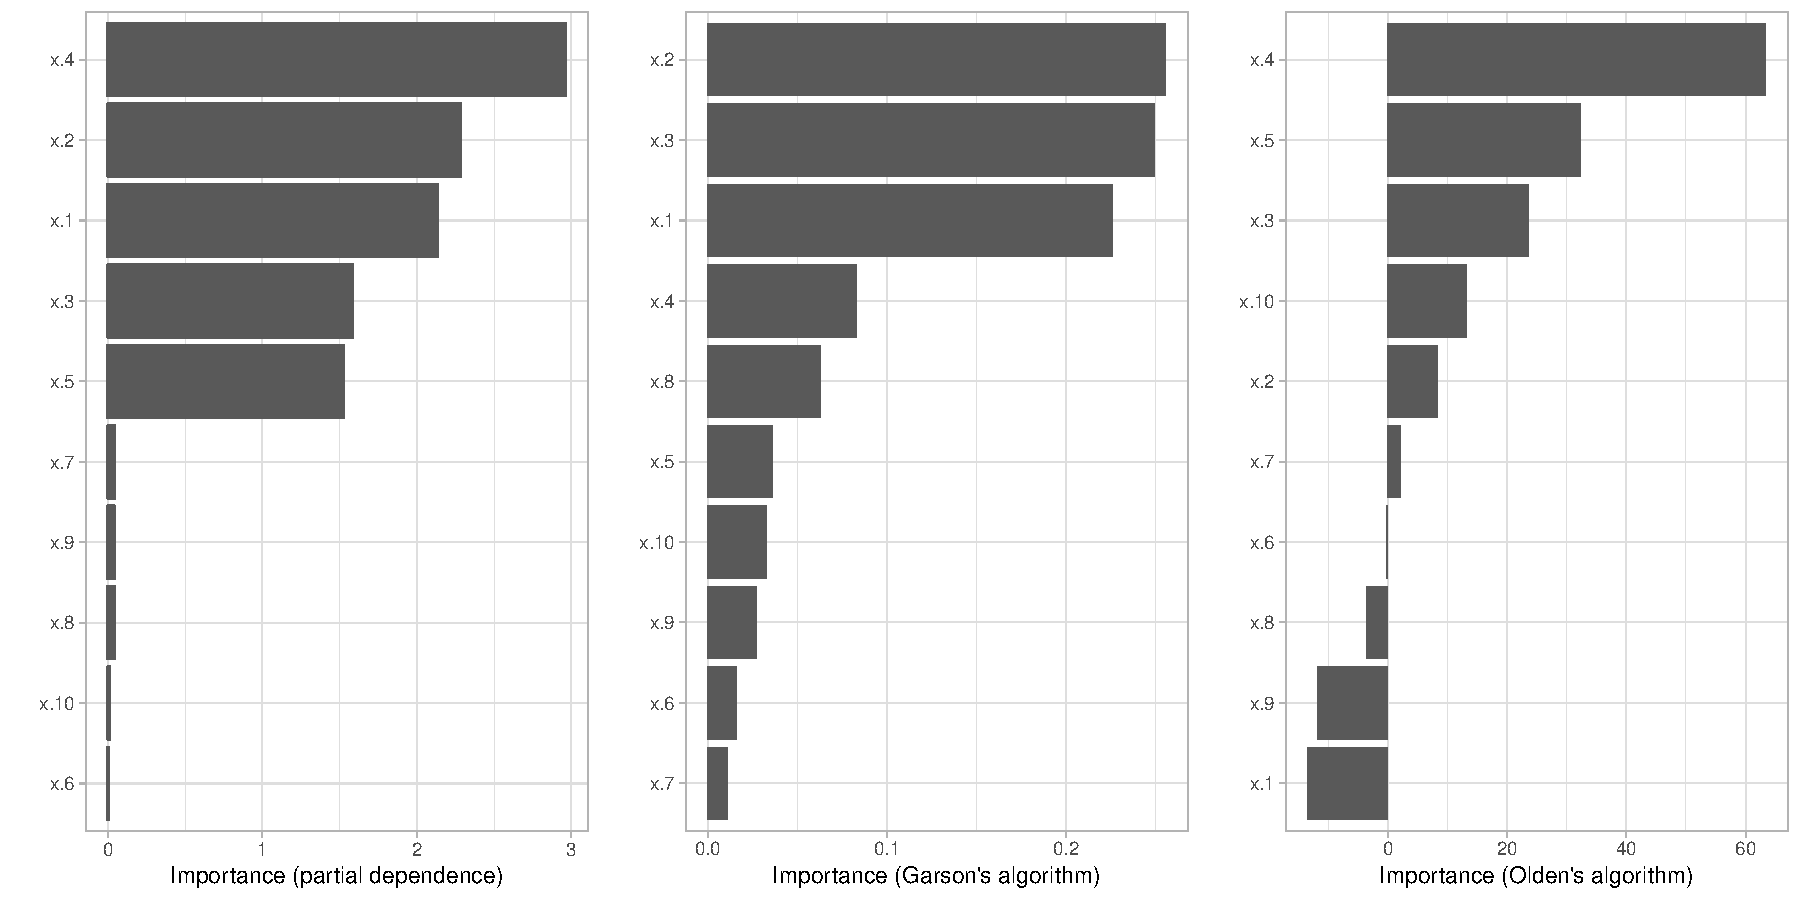
\includegraphics[width=1.0\textwidth]{network-vip}
  \caption{Variable importance plots neural network fit to the Friedman data set. \textit{Left}: partial dependence-based algorithm. \textit{Middle}: Garson's algorithm. \textit{Right}: Olden's algorithm. \label{fig:network-vip}}
\end{figure}

We also constructed the partial dependence functions for all pairwise interactions and computed the interaction statistic discussed in Section~\ref{sec:interaction}. The top ten interaction statistics are displayed in Figure~\ref{fig:network-int}. There is a clear indication of an interaction effect between the predictors $x_1$ and $x_2$, the only interaction present in the true model.

\begin{figure}[!htb]
  \centering
  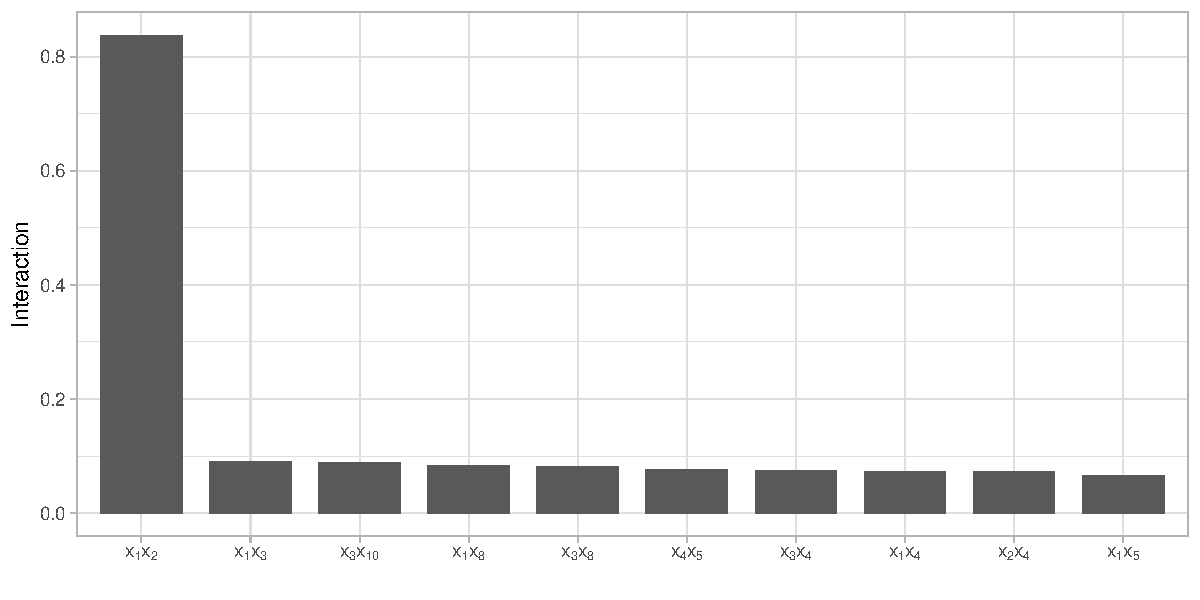
\includegraphics[width=0.75\textwidth]{network-int}
  \caption{Variable importance-based interaction statistics from the neural network fit to the Friedman data set. \label{fig:network-int}}
\end{figure}


%%%%%%%%%%%%%%%%%%%%%%%%%%%%%%%%%%%%%%%%%%%%%%%%%%%%%%%%%%%%%%%%%%%%%%%%%%%%%%%%
\subsubsection{Friedman's $H$-statistic}
%%%%%%%%%%%%%%%%%%%%%%%%%%%%%%%%%%%%%%%%%%%%%%%%%%%%%%%%%%%%%%%%%%%%%%%%%%%%%%%%

An alternative measure for the strength of interaction effects is known as Friedman's $H$-statistic \citep{friedman-2008-predictive}. Coincidentally, this statistic is also based on the partial dependence functions of the corresponding predictors, but uses a different approach.

For comparison, we fit a generalized boosted regression model (GBM) to the Friedman data set from the previous section. The parameters were chosen using 5-fold cross-validation. We used the R package \pkg{gbm} \citep{gbm-pkg} which has built-in support for computing Friedman's $H$-statistic for any combination of predictors. The results are displayed in Figure~\ref{fig:gbm-int}. To our surprise, the $H$-statistic did not seem to catch the true interaction between $x_1$ and $x_2$. Instead, the $H$-statistic ranked the pairs $\left(x_8, x_9\right)$ and $\left(x_7, x_10\right)$ as having the strongest interaction effects, but these predictors do not even appear in the true model. Our variable importance-based interaction statistic, on the other hand, clearly suggests that the pair $\left(x_1, x_2\right)$ has having the strongest interaction effect.

\begin{figure}[!htb]
  \centering
  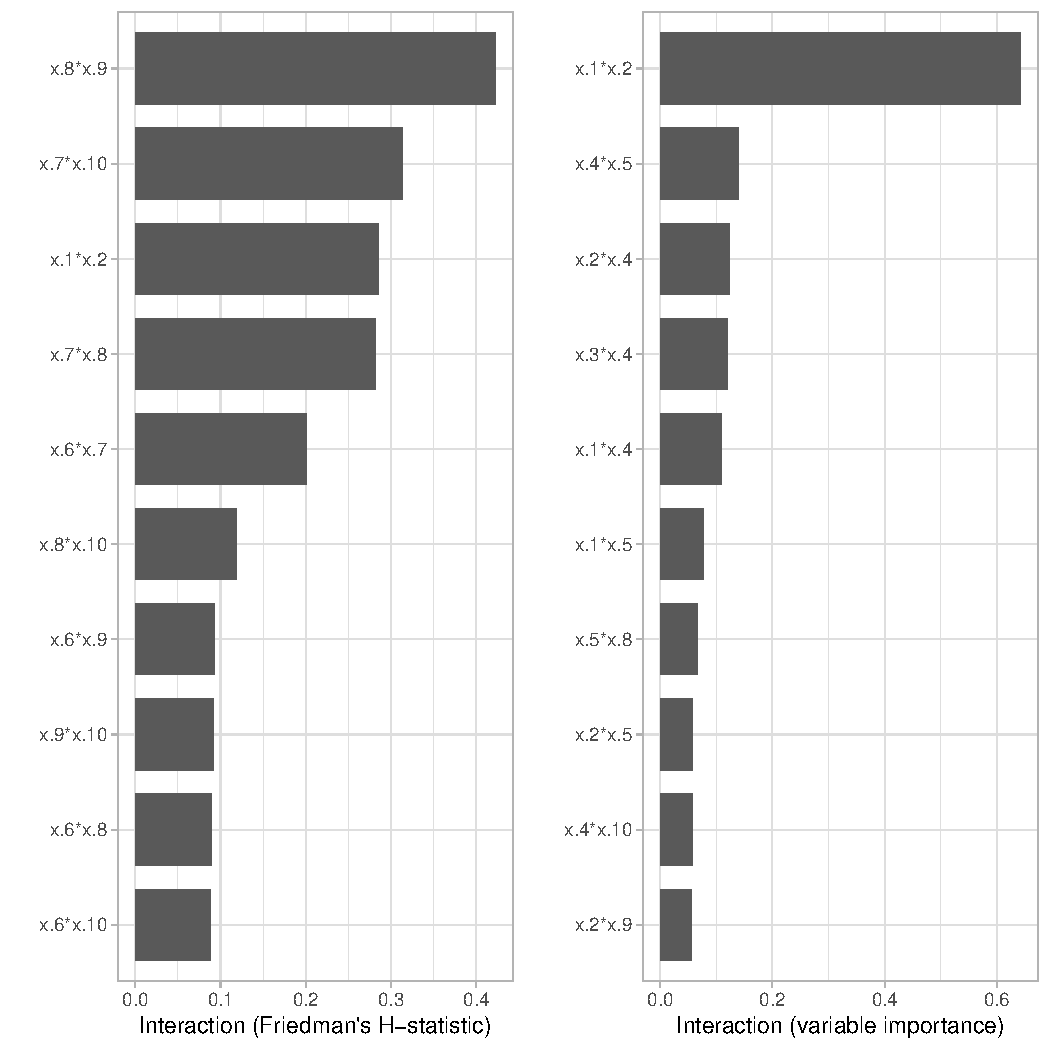
\includegraphics[width=0.75\textwidth]{gbm-int}
  \caption{Interaction statistics for the GBM model fit to the Friedman data set. \textit{Left}: Friedman's $H$-statistic. \textit{Right}: Our variable importance-based interaction statistic. \label{fig:gbm-int}}
\end{figure}


%%%%%%%%%%%%%%%%%%%%%%%%%%%%%%%%%%%%%%%%%%%%%%%%%%%%%%%%%%%%%%%%%%%%%%%%%%%%%%%%
\section{The Pima Indians diabetes data}
%%%%%%%%%%%%%%%%%%%%%%%%%%%%%%%%%%%%%%%%%%%%%%%%%%%%%%%%%%%%%%%%%%%%%%%%%%%%%%%%

In this section, we analyze the diabetes test results collected by the the US National Institute of Diabetes and Digestive and Kidney Diseases from a population of women who were at least 21 years old, of Pima Indian heritage, and living near Phoenix, Arizona. The data were taken directly from the \code{PimaIndiansDiabetes2} data frame which are available in the \pkg{mlbench} package \citep{mlbench-pkg}; for a description of the data and all the variables, see \url{https://archive.ics.uci.edu/ml/datasets/pima+indians+diabetes}.

We then used the \pkg{nnet} package \citep{venables-modern-2002} in R to fit a neural network with seven hidden units and a weight decay of 0.01; these parameters were chosen to maximize AUC using repeated 5-fold cross-validation with ten repeats; the cross-validated AUC was 0.77.

The partial dependence functions for all the predictors are displayed in Figure~\ref{fig:pima-pdps}. The PDPs clearly indicate that plasma glucose concentration (\code{glucose}), diabetes pedigree function (\code{pedigree}), and 2-hour serum insulin (\code{insulin}) have the largest effect on the neural network's prediction for the outcome of the diabetes test result (\code{diabetes}). On the other hand, the PDPs for diastolic blood pressure (\code{pressure}) and age (\code{age}) are relatively flat indicating they contribute less to the predictions than the other predictors. This is further illustrated in the variable importance plot displayed in Figure~\ref{fig:pima-vip}; the importance scores were obtained using Algorithm~\eqref{eqn:vi-con}.

\begin{figure}[!htb]
  \centering
  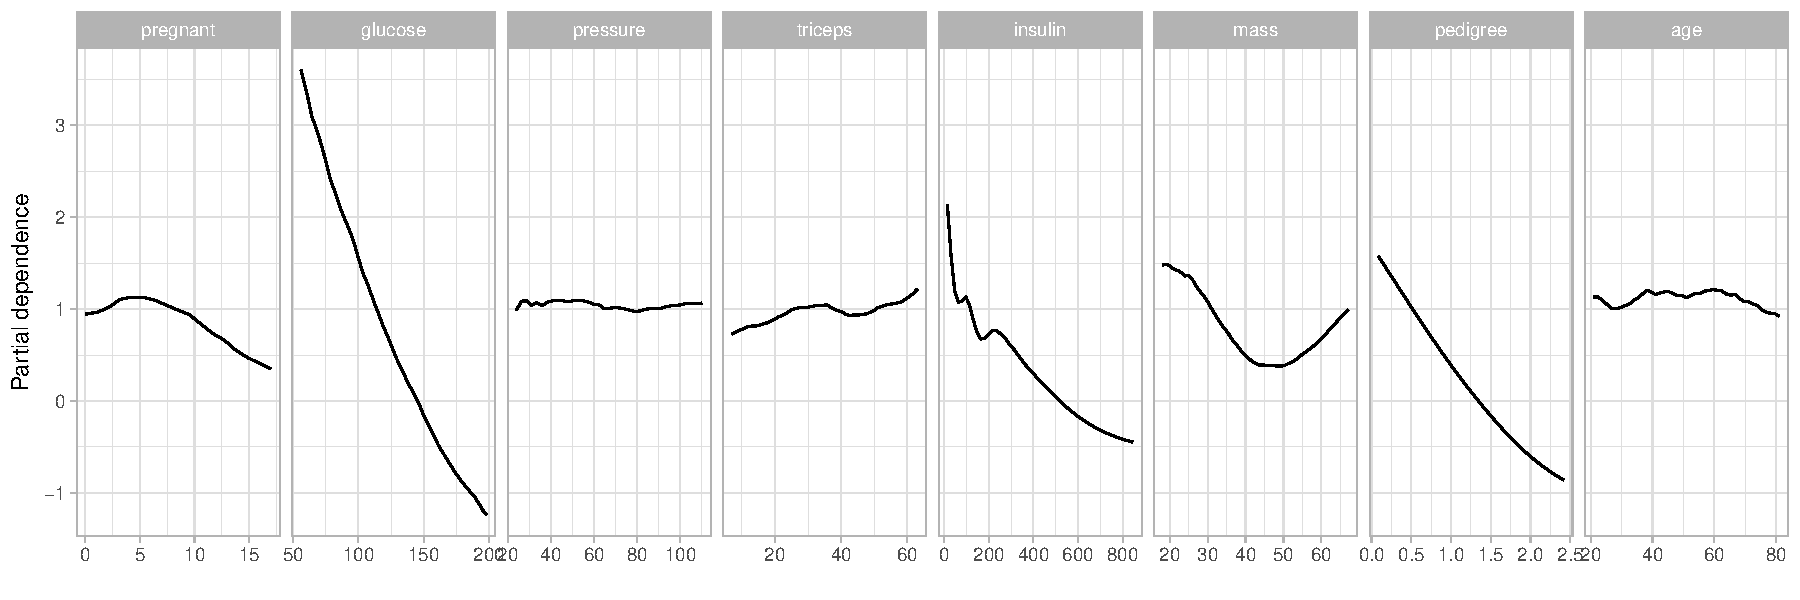
\includegraphics[width=1.0\textwidth]{pima-pdps}
  \caption{Partial-dependence plots for the eight predictors in the Pima Indians data set. \label{fig:pima-pdps}}
\end{figure}

\begin{figure}[!htb]
  \centering
  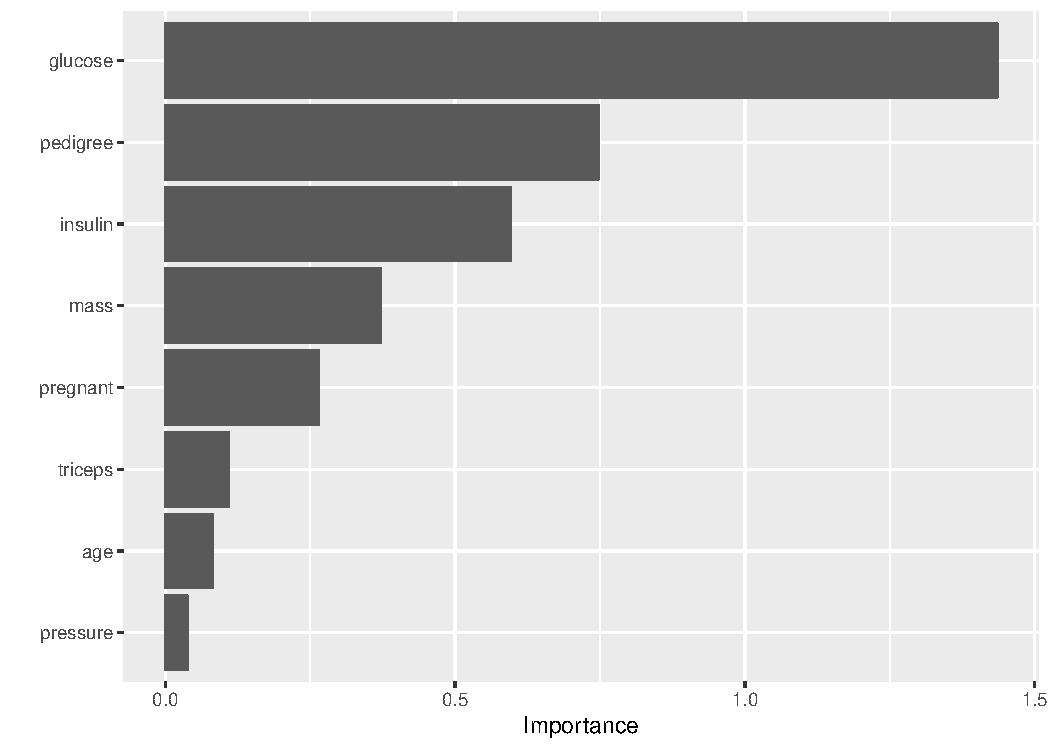
\includegraphics[width=1.0\textwidth]{pima-vip}
  \caption{Partial-dependence-based variable importance scores for the eight predictors in the Pima Indians data set. \label{fig:pima-vip}}
\end{figure}


%%%%%%%%%%%%%%%%%%%%%%%%%%%%%%%%%%%%%%%%%%%%%%%%%%%%%%%%%%%%%%%%%%%%%%%%%%%%%%%%
\section{Conclusion}
\label{sec:conc}
%%%%%%%%%%%%%%%%%%%%%%%%%%%%%%%%%%%%%%%%%%%%%%%%%%%%%%%%%%%%%%%%%%%%%%%%%%%%%%%%

We have discussed a new partial dependence-based variable important metric for supervised learning. Since our algorithm is based on Friedman's idea of partial dependence functions, our variable importance metric is model-based and takes into account the effects of the other features in the model. Consequently, this also requires that the fitted models be properly tuned to achieve optimum performance. We have also discussed a simple extension of our variable importance metric that seems useful for detecting interaction effects.

While this new approach to computing feature importance for any supervised learning algorithm seems very useful, more research is needed to determine where its deficiencies may lie. For example, outliers in the feature space can cause abnormally large fluctuations (outliers) in the partial dependence values $\bar{f}\left(x_{i}\right)$ $\left(i = 1, 2, \dots, k\right)$. Therefore, it may be advantageous to use more robust measures of spread to describe the variability in the estimated partial dependence function; a reasonable choice would be the median absolute deviation which has a finite sample breakdown point of $\floor{n / 2} / n$. It would also be interesting to see if our metric could be extended to rely on individual conditional expectation (ICE) curves \citep{goldstein-peeking-2015}, a refinement over Friedman's PDP.



%%%%%%%%%%%%%%%%%%%%%%%%%%%%%%%%%%%%%%%%%%%%%%%%%%%%%%%%%%%%%%%%%%%%%%%%%%%%%%%%
% Supplementary material
%%%%%%%%%%%%%%%%%%%%%%%%%%%%%%%%%%%%%%%%%%%%%%%%%%%%%%%%%%%%%%%%%%%%%%%%%%%%%%%%

\bigskip
\begin{center}
{\large\bf SUPPLEMENTARY MATERIAL}
\end{center}

\begin{description}

\item[R-package \pkg{vip}:] Contains function for computing variable importance scores and constructing variable importance plots for various types of fitted models in R. The package is hosted on GitHub at \url{https://github.com/AFIT-R/vip}.

\item{greenwell-vi-2017.R} R script containing the R code to reproduce all of the results and graphics in this paper.

\end{description}


%%%%%%%%%%%%%%%%%%%%%%%%%%%%%%%%%%%%%%%%%%%%%%%%%%%%%%%%%%%%%%%%%%%%%%%%%%%%%%%%
% Bibliography
%%%%%%%%%%%%%%%%%%%%%%%%%%%%%%%%%%%%%%%%%%%%%%%%%%%%%%%%%%%%%%%%%%%%%%%%%%%%%%%%

\bibliographystyle{Chicago}

\bibliography{greenwell-vi-2017}
\end{document}
